The primary objective of the Google Books project is to create a digital library
with global accessibility.~Through collaborations with libraries and publishers
worldwide, the project has amassed a collection of over 40 million books in more
than 400 languages. The process of adding a book to the digital library involves
several key steps, such as library registration, on-site visits by logistics
experts, and shipping the books for scanning. Therefore, the development of an
efficient scanning pipeline for global libraries requires meticulous planning
for optimal effectiveness. To address this challenge, Google invites
participants to create an efficient scanning pipeline for books, using a
scenario based on real-world circumstances as inspiration.

This problem revolves around two crucial components: libraries and books. The
central focus is on the books themselves, which require scanning. The primary
objective is to maximize the diversity of scanned books, each contributing a
specific score upon completion. On the other hand, libraries are characterized
by the collection of books they house and the rate at which they can dispatch
books for scanning. This implies that the number of books a library can scan per
day varies among different libraries. However, a library becomes operational for
book scanning only after completing a sign-up process that spans a certain
number of days.

\begin{figure}[h]
  \centering
  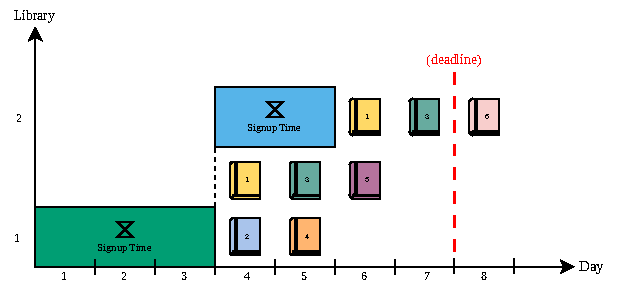
\includegraphics[width=\textwidth,keepaspectratio]{../assets/bs/bs-example.pdf}
  \caption{Book Scanning Process Example}
  \label{fig:bs-example}
\end{figure}